%%=============================================================================
% Template for Feber Reports in English
% for Bosch LaTeX Style v3.4
% Author:       Stephan.Simon@de.bosch.com                           2017-01-11
%%-----------------------------------------------------------------------------
% Copyright (c) 2001-2018 Robert Bosch GmbH and its subsidiaries.
% These LaTeX styles and templates and the accompanying materials are made
% available under the terms of the Bosch Internal Open Source License v4 which
% accompanies this distribution, and is available at
% http://bios.intranet.bosch.com/bioslv4.txt
%%=============================================================================
\documentclass[11pt,headings=small]{scrartcl}

% variable definitions are defined in this file:
%%
% This file contains the variable definitions for file
% PT_LOG_LISA_ScenarioBasedTotalDemandForecasting.tex
%%

\newcommand{\realnumbers}{\mathbb{R}}
\newcommand{\realnumbersnn}{\mathbb R_{\ge 0}}
\newcommand{\ts}{z}
\newcommand{\tstwo}{\textbf{z}}
\newcommand{\tssample}{\tilde{z}}
\newcommand{\tspoint}{\hat{z}}
\newcommand{\seriesiter}{i}
\newcommand{\buset}{\frak{B}}
\newcommand{\bu}{b}
\newcommand{\seriesset}{\frak{I}}
\newcommand{\seriessettrain}{\frak{I}^{\text{Tr}}}
\newcommand{\regionset}{\frak{R}}
\newcommand{\plantset}{\frak{W}}
\newcommand{\articleset}{\frak{A}}
\newcommand{\customerset}{\frak{C}}
\newcommand{\set}{\frak{I}}
\newcommand{\timeiter}{t}
\newcommand{\timeitermax}{T}
\newcommand{\timeiterzero}{t_{0}}
\newcommand{\condrange}{[1,\timeiterzero-1]}
\newcommand{\predrange}{[\timeiterzero,\timeitermax]}
\newcommand{\timerange}{[1,\timeitermax]}
\newcommand{\itspoint}{\tspoint^{\seriesiter}}
\newcommand{\itspointt}{\itspoint_{\timeiter}}
\newcommand{\tspointt}{\tspoint_{\timeiter}}
\newcommand{\its}{\ts^{\seriesiter}}
\newcommand{\itst}{\its_{\timeiter}}
\newcommand{\itstwo}{\tstwo^{\seriesiter}}
\newcommand{\itstwot}{\itstwo_{\timeiter}}
\newcommand{\covar}{\textbf{c}}
\newcommand{\icovar}{\covar^{\seriesiter}}
\newcommand{\icovart}{\icovar_{\timeiter}}
\newcommand{\itssample}{\tssample^{\seriesiter}}
\newcommand{\itssamplet}{\itssample_{\timeiter}}
\newcommand{\tssamplet}{\tssample_{\timeiter}}
\newcommand{\prob}{P}
\newcommand{\likelihood}{p}
\newcommand{\paramdist}{\theta}
\newcommand{\iparamdist}{\paramdist^{\seriesiter}}
\newcommand{\iparamdistt}{\iparamdist_{\timeiter}}
\newcommand{\paramNN}{\Theta}
\newcommand{\hiddenstate}{\textbf{h}}
\newcommand{\hiddenstatet}{\hiddenstate_{\timeiter}}
\newcommand{\ihiddenstate}{\hiddenstate^{\seriesiter}}
\newcommand{\ihiddenstatet}{\hiddenstatet^{\seriesiter}}
\newcommand{\hiddenstatefunction}{\frak{h}}
\newcommand{\horizon}{h}
\newcommand{\fcqualityweight}{w}
\newcommand{\ifcqualityweight}{\fcqualityweight_{\seriesiter}}
\newcommand{\price}{\frak{p}}
\newcommand{\iprice}{\price^{\seriesiter}}
\newcommand{\quantile}{u}
\newcommand{\quantiles}{\mathfrak{U}}
\newcommand{\identity}{\mathds{1}}
\newcommand{\quantileweight}{w^\quantiles}
\newcommand{\horizonweight}{w^\timeitermax}
\newcommand{\pastweight}{w^P}
\newcommand{\shrinking}{\gamma}
\newcommand{\RMSSE}{\textbf{RMSSE}}
\newcommand{\WRMSSE}{\textbf{WRMSSE}}
\newcommand{\normWRMSSE}{\textbf{normWRMSSE}}

\newcommand{\PL}{\textbf{PL}}
\newcommand{\SPL}{\textbf{SPL}}
\newcommand{\WSPL}{\textbf{WSPL}}

\newcommand{\RE}{\textbf{RE}}
\newcommand{\ARE}{\textbf{ARE}}
\newcommand{\TARE}{\textbf{TARE}}
\newcommand{\TRE}{\textbf{TRE}}
\newcommand{\maxtare}{\rho^\textbf{TARE}}
\newcommand{\maxtre}{\rho^\textbf{TRE}}
\newcommand{\FCA}{\textbf{FCA}}
\newcommand{\normFCE}{\textbf{normFCE}}
\newcommand{\FCB}{\textbf{FCB}}
\newcommand{\fcaweight}{\omega}
\newcommand{\OWE}{\textbf{OWE}}

\newcommand{\mean}{\mu}
\newcommand{\shape}{\alpha}
\newcommand{\likelihoodnn}{\likelihood_{NB}}

\newcommand{\nnweight}{\textbf{w}}
\newcommand{\nnthreshold}{b}

\newcommand{\loglikelihood}{\mathcal{L}}
\newcommand{\scalefactor}{\nu}
\newcommand{\iscalefactor}{\scalefactor^{\seriesiter}}

\usepackage{cite}
\usepackage{subcaption}
\usepackage{dsfont}
\usepackage{mathtools}
\usepackage[english]{babel} % for English text only
%\usepackage[ngerman]{babel} % for German text only
%\usepackage{ngerman}        % for German text only
\usepackage[T1]{fontenc}
\usepackage[utf8]{inputenc}
\usepackage{microtype} % improves font spacing, needs pdfTEX >= 1.20
%\usepackage{amsmath}
\usepackage{lipsum}% delete this package and the \lipsum commands

% Bosch style and its primary options, COMMA-SEPARATED, NO EMPTY LINES!
% If you are unsure about an option: just comment it out, defaults exist!
\usepackage[
% The language setting affects some text labels:
% Language = { English | German }
Language = English,
%
% Frequently used page formats:
% Format = { A4portrait | A4landscape | 16to10 | 16to9 }
Format = A4portrait,
%
% Sans serif font "Bosch Office Sans" or serif font "Utopia":
% isSerif = { false | true }
isSerif = true,
%
% Base color (affects titles and some color boxes):
% BaseColor = { Fuchsia | Violet | DarkBlue | LightBlue | Turquoise |
%               LightGreen | DarkGreen | Gray}
BaseColor = LightBlue,
%
% Color of the Bosch Supergraphic:
% SgColor = { Multi | DarkBlue | LightBlue | Green | Red | Violet |
%             DarkGray | MediumGray | LightGray }
SgColor = Multi,
%
% Placement of Supergraphic in header, optionally LifeClip, optionally slogan:
% SgPlace = { Top | Bottom | Fill | FillSlogan}
SgPlace = Bottom,
%
% Background of header { Empty | White | Gray | Super }
HeaderBg = Gray,
%
% Shall title A and title B be in the same line to save space:
% isShallowTitle = { false | true }
isShallowTitle = false,
%
% Whitespace at top edge of page (in 1/40 of paperheight units, usually 0)
TopWS = 0,
% Whitespace at bottom of page (in 1/40 of paperheight units, usually 1)
BottomWS = 1,
%
% Is whitespace at left/right edge of page or does the header use this space:
% isLeftWS = { false | true }
isLeftWS = false,
isRightWS = false,
%
% Eye catcher picture may be absent or included in a pre-defined height:
% EyeCatcherMode = { None | Tiny | Small | Medium | Large }
EyeCatcherMode = Tiny,
%
% Shrink logo: How often does the height of H in BOSCH fit into page diagonal:
% 54 (large, for self-printed communication) or 98 (small, like PPT-template)
NumOfHinDiag = 85,
%
% Relative height of SuperStripe, percentage of height of H in BOSCH
SuperStripeHeightPercentOfH = 100,
%
% Height of header (in 1/40 of paperheight units) in portrait/landscape mode
HeadHeightPortrait = 4,
HeadHeightLandscape = 5,
%
% Horizontal space, left and right border (in 1/40 of paperwidth units)
HorzSpacePortrait = 2,
HorzSpaceLandscape = 1.5,
%
% Vertical space, top and bottom border (in 1/40 of paperheight units)
VertSpacePortrait = 1,
VertSpaceLandscape = 1.5,
%
% For LaTeX developers: draw a testgrid (40 x 40 rectangles):
% isGrid = { false | true }
isGrid = false,
]{bosch}
% Invoke the universal Bosch report pagestyle.
\pagestyle{boschrep}

%%-----------------------------------------------------------------------------
% Customization of bosch style.
% Any customization lines can be deleted if not needed!
% Leaving the arguments empty yields the same result except page numbering
% with \RBpage{} which is disabled by empty argument.
%%-----------------------------------------------------------------------------
% confidentiality class from -1 (no footer) to 3 (strictly confidential)
\RBconfidentiality{1}

\RBtitleA{PT-LOG LISA Scenario-Based Total Demand Forecasting}

\RBversion{}
\RBdate{}% leave empty to set date automatically
\RBpage{LinkLast}% { | Simple | Last | LinkLast }

% you can specify an eye catcher picture here
%\RBmyPic{14080928EmptyRoad}
\RBmyPic{140823186EmptyRoad}

% First author name (A), department, phone.  Only author A's name is printed in
% the header.  You may change this header information from page to page.
% Alternatively, you may put several authors names into field A and leave B and
% C empty.  This is also the recommended solution if you have more than three
% authors.
\RBauthorA{Dr. Oliver Hoenig}
\RBdepartmentA{PT/LOI1}
%\RBphoneA{+49 5121 49 0000}

% Second author name (B) (if empty: table element not printed), department.
\RBauthorB{Dr. Daniel Stanek}
\RBdepartmentB{PT/LOI1}

% Second author name (C) (if empty: table element not printed), department.
\RBauthorC{Dr. Najdan Vukovic}
\RBdepartmentC{CI/DAP41.7}

%%-----------------------------------------------------------------------------
% FEBER-specific settings with their default settings. Uncomment as necessary.
%%-----------------------------------------------------------------------------
% Use sub-title and extra footer field for FEBER-specific information
\RBfeberSetup

\RBexportControlRelevant{No} % won't compile if this is undefined!

\RBreportNumber{}

% Standard report types are "Final Report", "Service", "Project", "Study",
% "Preliminary Work" and "Interim Report".
% In German: "Abschlussbericht", "Dienstleistung", "Projekt", "Studie",
% "Vorarbeit" and "Zwischenbericht".
\RBreportType{Interim Report}

%\RBenclosures{No}
%\RBexternalReleaseCover{No}
%\RBexternalReleaseEnclosures{No}
%\RBresponsiblePerson{}
%\RBresponsiblePersonOrg{}
%\RBreviewer{}
%\RBreviewerOrg{}
%\RBreleasingPersonA{}
%\RBreleasingPersonAOrg{}
%\RBreleasingPersonB{}
%\RBreleasingPersonBOrg{}
%\RBreleasingPersonC{}
%\RBreleasingPersonCOrg{}
%\RBrecipients{}
%\RBcC{}
%\RBkeywords{}

%%-----------------------------------------------------------------------------
% Other customization - taste-dependent ...
%%-----------------------------------------------------------------------------
% numbering depth for headings and table of contents
\setcounter{secnumdepth}{3}
\setcounter{tocdepth}{2}

% Formatting (see Klöckl, p.77)
\setcounter{topnumber}{5}           % max num. of floats at head
\setcounter{bottomnumber}{5}        % max num. of floats at foot
\setcounter{totalnumber}{10}        % max num. of floats
\renewcommand{\topfraction}{1.0}    % max. part of floats at head
\renewcommand{\bottomfraction}{1.0} % max. part of floats at foot
\renewcommand{\textfraction}{0.0}   % min. part of text
\renewcommand{\dbltopfraction}{1.0} % for wide floats in twocolumn
\renewcommand{\floatpagefraction}{1.0} % must be filled before new floats page
\renewcommand{\dblfloatpagefraction}{1.0} % for wide floats in twocolumn

% Naming of figures
\addto\extrasenglish{\renewcommand{\figurename}{Fig.}}
\addto\extrasngerman{\renewcommand{\figurename}{Fig.}}
\newcommand{\Fig}{Fig.\xspace}
\newcommand{\Abb}{Abb.\xspace}

%%-----------------------------------------------------------------------------
% Your own shortcuts and commands
%%-----------------------------------------------------------------------------

% Trennregeln
\hyphenation{}

%%-----------------------------------------------------------------------------
% Document begins here
%%-----------------------------------------------------------------------------
\begin{document}


%\twocolumn% outcomment if you prefer one column


\begin{abstract} 
	
The supply chain of Robert Bosch Power Tools is characterized by short lead-times to its customers (48hours) but long replenishment, production and supplier lead times (up to 18 months). Therefore a precise demand forecast is crucial. This is currently done in a standard demand managment software which creates point forecasts of all forecast relevant base combinations up to the next 24 months. These are then fed into a inventory management system which calculates the optimal stock level and derives and automatically triggers then replenishment decisions using a complex reorder point heuristic.  The product \textit{Scenario-Based Total Demand Forecasting} of the PT-LOG program \textit{LISA} calculates distribution forecasts of the total demand of all forecast relevant base combinations up to the next 18 months. Certain percentiles of these distributions are then loaded into the standard demand planning system of PT. These demand distribution forecasts can then be used downstream to more precisely optimize replenishment and inventory decisions.

\end{abstract}

\section{Introduction}
\label{section:Intro}


[X longer part about the setup and circumstancence of the LISA project and PT planning X]

This report is structured as follows. We begin by reviewing related work in Section \ref{section:Rel} before we introduce our approach in Section \ref{section:Model}. Then we introduce how the model perfromance is evaluated in Section \ref{section:Perf}. Afterwards we describe our implementation in Section \ref{section:Impl} and show our results in Section \ref{section:Res}. Next, we describe possible future steps in Section \ref{section:Future}. We finish with a conclusion in Section \ref{section:Concl}.




\section{Related Work}
\label{section:Rel}

\section{Model}
\label{section:Model}

The entities of multi-variate time series will be denoted $\itst\in\realnumbersnn$ for series $\seriesiter \in \seriesset$ and time $\timeiter \in \timerange$.
 
The series set $\seriesset$ consists of all forecast relevant base items 
$\seriesset = X_{\bu\in\buset} \seriesset_{\bu} = \times_{\bu\in\buset}\articleset_{\bu} \times \plantset \times \regionset \times \customerset$ where $\times$ denotes the cross product of sets, $\buset$ is the set of Business Units, $\seriesset_{\bu}$ is the set of forecast relevant base types for Business Unit $\bu$, $\articleset_{\bu}$ denotes the set of articles belonging to Business Unit $\bu$, $\plantset$ denotes the set of warehouses, $\regionset$ denotes the set of regions like a regional sales organisation RSO or a country sales organisation CSO, and  $\customerset$ denotes the set of customer groups.

The time interval $\timerange$ can be split into a conditioning range $\condrange$ and a prediction range $\predrange$. In the conditioning range the time series values are known, in the prediction range the time series values are unkown or at least to be predicted. We make sure that each time series $\seriesiter \in \seriesset$ has data within the full conditioning range $\condrange$ by filling up shorter time series by leading Zeros.

In addition to the time series values itself $\itst$ we also have $m$-dimensional covariates $\icovart\in\realnumbers^{m}$ for series $\seriesiter \in \seriesset$ and time $\timeiter \in \timerange$. It is assumed that the covariate values are both known for the conditioning range and a prediction range.

The goal is to predict the conditional probabilities

\begin{equation}\label{condprob}
\prob \left( \its_{\predrange} \Big| \its_{\condrange} , \icovar_{\timerange} \right) \quad \forall \seriesiter \in \seriesset
\end{equation}

We assume that at each time step the values are drawn in an independent and identically distributed way. Then Eq. (\ref{condprob}) can be expanded as an autoregressive product

\begin{equation}\label{condprobiid}
\prob \left( \its_{\predrange} \Big| \its_{\condrange} , \icovar_{\timerange} \right) = \prod_{\timeiter=\timeiterzero}^{\timeitermax} \prob \left( \its_{\timeiter} \Big| \its_{[1,\timeiter-1]} , \icovar_{\timerange} \right) \quad \forall \seriesiter \in \seriesset
\end{equation}


We are currently working on two approaches which are introduced now.

\subsection{Approach 1: DeepAR: Probabilistic forecasting with autoregressive recurrent networks}
\label{subsection:deepar}

For the first approach we orientate us at Ref. \cite{SALINAS20201181} and \cite{DBLP:journals/corr/abs-1906-05264} and the model is summarized in Fig. \ref{fig:DeepAR}. The model is based on the ideas of Ref. \cite{DBLP:journals/corr/Graves13} and \cite{DBLP:journals/corr/SutskeverVL14}.

\begin{figure}
	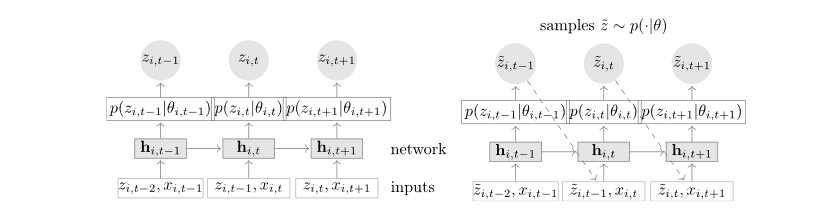
\includegraphics[width=\linewidth]{pics/RNN_DeepAR.png}
	\caption{Figure 3 from Ref. \cite{SALINAS20201181}. Summary of the model: Training is shown on the left, prediction is shown on the right. At each time step $\timeiter$, the inputs to the network are the covariates $\icovart$, the target value at the previous time step $\its_{\timeiter-1}$, and the previous network output $\ihiddenstate_{\timeiter-1}$. The network output $\ihiddenstatet =  \hiddenstatefunction \left(\ihiddenstate_{\timeiter-1},\its_{\timeiter-1},\icovart,\paramNN   \right)$ is then used to compute the parameters $\iparamdistt=\paramdist(\ihiddenstatet,\paramNN)$ of the likelihood $\likelihood(\ts|\paramdist)$, which is used for training the model parameters. For prediction, the history of the time series $\itst$ is fed in for $\timeiter<\timeiterzero$, then in the prediction range (right) for $\timeiter\ge\timeiterzero$ a sample $\itst \sim \likelihood(.|\iparamdistt)$ is drawn and fed back for the next point until the end of the prediction range, generating one sample trace. Repeating this prediction process yields many traces that represent the joint predicted distribution.}
	\label{fig:DeepAR}
\end{figure}

\subsubsection{Model}
\label{subsection:approach1model}


Starting at Eq. (\ref{condprobiid}), we further assume that the conditional probabilities at each time step can be modeled as likelihood factors

\begin{equation}\label{likelihood}
\prob \left( \its_{\timeiter} \Big| \its_{[1,\timeiter-1]} , \icovar_{\timerange} \right) =
\likelihood \left( \its_{\timeiter} \Big| \paramdist(\ihiddenstatet,\paramNN) \right)
\end{equation}

where $\paramdist$ models a function which outputs all parameters of the likelihood distribution. It is parametrized by the output of an \textbf{autoregressive recurrent network}

\begin{equation}\label{hiddenstate}
\ihiddenstatet =  \hiddenstatefunction \left(\ihiddenstate_{\timeiter-1},\its_{\timeiter-1},\icovart,\paramNN   \right)
\end{equation}

where $\hiddenstatefunction$ is a function which is implemented by a \textbf{multi-layer recurrent neural network with LSTM cells} parametrized by $\paramNN$.

The likelihood $\likelihood \left( \its_{\timeiter} \Big| \paramdist(\ihiddenstatet,\paramNN) \right)$ (as a function of $\paramdist$ for a fixed $\its_{\timeiter}$) is a fixed distribution with parameters that come out of the function $\paramdist(\ihiddenstatet,\paramNN)$.

In the original sequence-to-sequence setup of Ref. \cite{DBLP:journals/corr/Graves13} and \cite{DBLP:journals/corr/SutskeverVL14}, there is a encoder network learned on the training range and a decoder network learned on the prediction range. In our context based on Ref. \cite{SALINAS20201181}, these two networks are identical in architecture and parameters $\paramNN$.  The initial states of the encoder $\ihiddenstate_{0}$ and $\its_{0}$ are initialized to zero. The initial hidden state of the decoder $\ihiddenstate_{\timeiterzero-1}$ is obtained by computing Eq. (\ref{hiddenstate}) for $\timeiter\in\condrange$, where all required quantities are observed.

With trained network parameters $\paramNN$, we can than draw joint samples $\itssample_{\predrange} \sim \prob \left( \its_{\predrange} \Big| \its_{\condrange} , \icovar_{\timerange} \right)$ by ancestral sampling. By drawing many of these joint samples we can calculate the quantiles of interest. 


\subsubsection{Likelihood function}
\label{subsubsection:App1likelyhood}

The likelihood $\likelihood(\ts|\paramdist)$ defines the "noise model" and it should match the data as close as possible. It models the probability distribution of the time series value in the next time step. All parameters  of the likelihood are a direct outcome out of the neural network.

Many likelihood models are possible in this context as long as samples from the distribution can be obtained cheaply, and the log-likelihoodand its gradients with respect to the parameters can be evaluated.

In our case of sales quantities $\itst\in\realnumbersnn$, the negative-binomial likelihood is a good choice, see e.g. Ref. \cite{10.5555/3044805.3045048} or \cite{SNYDER2012485}.

We parameterize the negative binomial distribution by its mean $\mean\in\realnumbersnn$ and its shape parameter $\shape\in\realnumbersnn$,

\begin{equation}\label{nonnegativebinomial}
\likelihoodnn(\ts|\mean,\shape) = \frac{\Gamma(\ts + \frac{1}{\shape})}{\Gamma(\ts + 1)\Gamma(\frac{1}{\shape})}\left(\frac{1}{1+\shape\mean}\right)^{\frac{1}{\shape}}\left(\frac{\shape\mean}{1+\shape\mean}\right)^{\ts}
\end{equation}

with

\begin{subequations}\label{nonnegativebinomialparameters}
	\begin{align}
	\mean &= \mean(\ihiddenstatet) = \log\left(1 + \exp\left(\nnweight^{T}_{\mean}\ihiddenstatet + \nnthreshold_{\mean}\right)\right)\\
	\shape &= \shape(\ihiddenstatet) = \log\left(1 + \exp\left(\nnweight^{T}_{\shape}\ihiddenstatet + \nnthreshold_{\shape}\right)\right)
	\end{align}
\end{subequations}


where both parameters are obtained from the network output by a fully-connected layer with softplus activations as to ensure positivity. In this parameterization of the negative binomial distribution, the shape parameter $\shape$ scales the variance relative to the mean, i.e. $Var[\ts] = \mean+\mean^{2}\shape$.

\subsubsection{Training}
\label{subsubsection:App1Training}
For the training, we define the loglikelihood function as

\begin{equation}\label{loglikelihood}
\loglikelihood = \sum_{\seriesiter\in\seriessettrain}\sum_{\timeiter=\timeiterzero}^{\timeitermax}\log(\likelihood(\its_{\timeiter} | \paramdist(\ihiddenstatet,\paramNN)))
\end{equation}

with $\seriessettrain$ as the training set where $\itst$ and $\icovart$ is known for all $\timeiter\in[1,\timeitermax]$ and $\seriesiter\in\seriessettrain$. The loglikelihood function is now maximized with respect to $\paramNN$, all parameters of $\hiddenstatefunction(.)$ and $\paramdist(.)$. The optimization can be done directly via stochastic gradient descent by computing gradients with respect to  $\paramNN$. As here, encoder and decoder is identical, we can set $\timeiterzero$ to Zero in Eq. (\ref{loglikelihood}) such that we optimize over the condition and prediction range. For each timeseries in the dataset $\seriesset$, we generate multiple training instances by selecting from the original timeseries windows with different starting points but  total length $\timeitermax$ and the relative lengths of the conditioning and prediction ranges fixed for all training examples. We allow also start points before the beginning of a given timeseries and fill up the missing points with Zeros. By this, the model can learn also pattern for new items.

\subsubsection{Scale handling}
\label{subsubsection:App1lScaleHandling}

Our time series despict a power law, so we have many tiny time series and a few very big ones. Out of this two problems arise, see Ref. \cite{SALINAS20201181}.

Firstly, the autoregressive nature of the model means that the input and output scales directly with the time series values but the non-linearities of the network in between have only a limited operating range. Therefore the neural net would need to learn additional mappings which is hard. Ref. \cite{SALINAS20201181} addresses this issue by dividing the autoregressive inputs $\its$ by an item-dependent scale factor $\iscalefactor$, and conversely multiplying the scale-dependent likelihood parameters by the same factor. The negative binomial likelihood parameters of Eq. (\ref{nonnegativebinomialparameters}) become

\begin{subequations}\label{nonnegativebinomialparametersscaled}
	\begin{align}
	\mean &= \iscalefactor\log\left(1 + \exp\left(\nnweight^{T}_{\mean}\ihiddenstatet + \nnthreshold_{\mean}\right)\right)\\
	\shape &= \frac{\log\left(1 + \exp\left(\nnweight^{T}_{\shape}\ihiddenstatet + \nnthreshold_{\shape}\right)\right)}{\sqrt{\iscalefactor}} 
	\end{align}
\end{subequations}

A practical solution in Ref. \cite{SALINAS20201181} for the item-dependent scale factor $\iscalefactor$ is to use the time series average

\begin{equation}\label{scalefactor}
\iscalefactor = 1 + \frac{1}{\timeiterzero}\sum_{\timeiter=1}^{\timeiterzero}\itst
\end{equation}

The second problem is that the imbalance in the data means that a stochastic optimization procedure that picks training instances uniformly at random will visit the small number time series with large scales very infrequently, resulting in those time series being underfitted. In our demand forecasting setting often these large scale time series show different behaviour. This is than not learned enough by the model, exactly there were it is most important as these time series represent the highest business value. Ref. \cite{SALINAS20201181} solves this by using a weighted sampling scheme that sets the probability of selecting a window from an example with scale $\iscalefactor$ proportional to $\iscalefactor$.


\subsection{Approach 2: Multi-variate Probabilistic Time Series Forecasting via Conditioned Normalizing Flows}
\label{subsection:zalando}

For the second approach we orientate us at Ref. \cite{rasul2020multivariate}. 

\subsubsection{Differences between the two Approaches}
\label{subsubsection:diffapproach}

The main differences to the first approach (based on Ref. \cite{SALINAS20201181}) are
\begin{itemize}
	\item In the second approach all time series are modelled joinly as one complex multi-variate probability distribution (each time series is one addtional dimension) while in the first approach there is only one scalar probability distribution which needs to fit for all time series. This enables the model to take effects like cannibalization and other cross-time series effects into account.
	\item In the second approach using conditional normalized flows (see Ref. \cite{papamakarios2018masked} and \cite{DBLP:journals/corr/DinhSB16}) the distribution can be arbitrarily complex while in the first approach one has to choose one distribution class for all time series, e.g. nonnegative binomial for count data.
	\item Instead of an RNN with LSTM cells in approach 1, here one can use either a RNN with GRUs (see Ref. \cite{DBLP:journals/corr/ChungGCB14}) or a Transformer model using Self-Attention (see Ref. \cite{DBLP:journals/corr/VaswaniSPUJGKP17})
	\item For categorical features of the covariates approach 2 uses embeddings (see Ref. \cite{DBLP:journals/corr/GuoB16})
\end{itemize}

\subsubsection{Model}
\label{subsection:approach2model}

\begin{figure}
	\centering
	\begin{subfigure}{.5\textwidth}
		\centering
		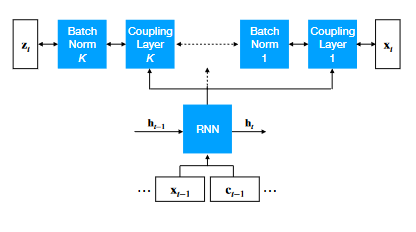
\includegraphics[width=.95\linewidth]{pics/RNN_NormFlow_Zalando.png}
		\caption{Fig 1 of Ref. \cite{rasul2020multivariate}: RNN Conditioned Real NVP model schematic at time $\timeiter$, consisting of K blocks of coupling layers and Batch Normalization,  where in each coupling layer we condition the time series (in the pic denoted $x_t$) and its transformations on the state of a shared RNN from the previous time step and its covariates which are typically timedependent and time independent features.}
		\label{fig:subfig:RNN_NormFlow_Zalando}
	\end{subfigure}%
	\begin{subfigure}{.5\textwidth}
		\centering
		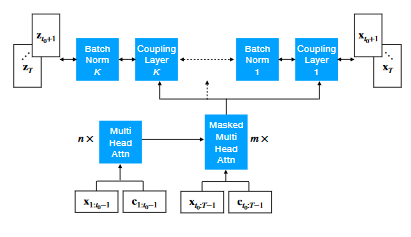
\includegraphics[width=.95\linewidth]{pics/Transformer_NormFlow_Zalando.png}
		\caption{Fig 2 of Ref. \cite{rasul2020multivariate}: Transformer Conditioned Real NVP model schematic consisting of an encoder-decoder stack where the encoder takes in some context length of time series and then uses it to generate conditioning for the prediction length portion of the time series via a causally masked decoder stack. The output of the decoder is used as conditioning to train the flow. Note that the positional encodings are part of the covariates and unlike the RNN model,here all time series time points are trained in parallel.}
		\label{fig:subfig:Transformer_NormFlow_Zalando}
	\end{subfigure}
	\caption{The two main different model architectures of approach 2 based on Ref. \cite{rasul2020multivariate}}
	\label{fig:Approach2}
\end{figure}

The goal is to predict the conditional probability 

\begin{equation}\label{condprob}
\prob \left( \tstwo_{\predrange} \Big| \tstwo_{\condrange} , \covar_{\timerange} \right)
\end{equation}
where $\tstwo = [\its]_{\seriesiter\in\seriesset}$ is the multi-variate time series vector and $\covar=\{\icovar\}_{\seriesiter\in\seriesset}$ are the covariates over all times series.

Fig. \ref{fig:Approach2} shows schematically the 2 possible architectures within the second approach.



\subsubsection{Conditioned Real NVP}
\label{subsection:approach2condflow}
 
Based on Ref. \cite{papamakarios2018masked} and \cite{DBLP:journals/corr/DinhSB16} the 2nd approach uses conditioned real non-volume preserving flows (Real NVP) in order to model complex multi-dimensional density distributions. Fig. \ref{fig:RealNVP} describes the main idea.

\begin{figure}
	\centering
	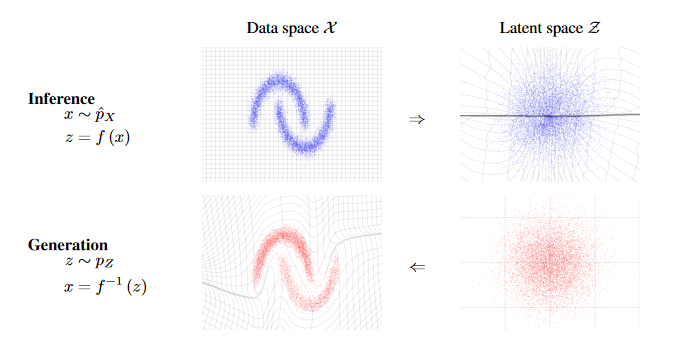
\includegraphics[width=.9\linewidth]{pics/RealNVP.png}
	\caption{Fig. 1 from Ref. \cite{DBLP:journals/corr/DinhSB16}. Real NVP learns an invertible, stable, mapping between a data distribution and a latent distribution (typically a Gaussian).}
	\label{fig:RealNVP}
\end{figure}



\section{Performance Evalution}
\label{section:Perf}

In this section, we define how we evaluate the performance of our solution.

\subsection{Forecast Horizon}
\label{subsection:ForecastHorizon}

In the first phase, we forecast 6 months ahead. All horizons will be weighted equally in the performance evaluation:

\begin{equation}\label{horizonweigths}
\horizonweight_\timeiter = \frac{1}{\timeitermax - \timeiterzero}\quad \forall \timeiter\in\predrange.
\end{equation}

\subsection{Historic Horizon}
\label{subsection:HistoricHorizon}

We will use the last 24 months to condition our model. In addition we will use this data also to scale our errors using the following weights

\begin{equation}\label{pastweigths}
\pastweight_\timeiter = \frac{\shrinking ^{\timeiterzero - 1 - \timeiter}}{\sum_{r=2}^{\timeiterzero - 1}\shrinking ^{\timeiterzero - 1 - r}}  \quad \forall \timeiter\in[2,\timeiterzero-1].
\end{equation}

$\shrinking\in[0,1]$ is a shrinkage factor which reduces the weights for times farer in the past. Here we will use  $\shrinking=0.95$.

\subsection{Point Forecast}
\label{subsection:PointForecast}

Even when our goal is to forecast the demand density, we will measure a forecast quality on a point forecast to compare the new solution with our existing benchmark solutions. We use the median to map the density to a point:

\begin{equation}\label{pointforecast}
\itspointt = \itspointt (0.5)  =  Median\left(\prob \left( \its_{\timeiter} \Big| \its_{[1,\timeiter-1]} , \icovar_{\timerange} \right)\right)
\end{equation}

\subsubsection{Root Mean Squared Scaled Error}
\label{subsubsection:RootMeanSquaredScaledError}

Then for the forecast quality measure, we use the Root Mean Squared Scaled Error (\RMSSE) as in REf. \cite{M5Competition}:

\begin{equation}\label{RMSSE}
\RMSSE^{\seriesiter} =  \sqrt{\frac{\sum_{\timeiter=\timeiterzero}^{\timeitermax} \horizonweight_\timeiter \left(\its_{\timeiter} - \itspointt \right)^{2} }{\sum_{\timeiter=2}^{\timeiterzero - 1}\pastweight_\timeiter\left(\its_{\timeiter} - \its_{\timeiter-1} \right)^{2}}}
\end{equation}

where $\its_{\timeiter}$ is the actual value of the time series $\seriesiter$ at time $\timeiter$, $\horizonweight_\timeiter$ is the horizon weight from Eq. (\ref{horizonweigths}) and $\pastweight_\timeiter$ is the past weight from Eq. (\ref{pastweigths}). 

The nominator of Eq. (\ref{RMSSE}) can be also interpreted as the expected weighted average forecast error using the naive forecasting method $\itspointt = \its_{\timeiter-1}$. Therefore, $\RMSSE$ can interpreted as the ratio of the weighted average forecasting error over the prediction range of our forecast vs the expected (based on the past) weighted average forecast error using the naive forecasting.

For the forecast quality measure of a set of forecasts we use the \textbf{Weighted \RMSSE(\WRMSSE}),

\begin{equation}\label{WRMSSE}
\WRMSSE = \sum_{\seriesiter\in\seriesset} \ifcqualityweight \RMSSE^{\seriesiter} 
\end{equation}

where $\ifcqualityweight$ are the weights for each series defined by 

\begin{equation}\label{fcqualityweight}
\ifcqualityweight = \frac{\iprice * \left(\sum_{\timeiter=1}^{\timeiterzero-1}\pastweight_\timeiter\its_{\timeiter}\right)}{
	\sum_{j\in\seriesset}\price^{j} * \left(\sum_{\timeiter=1}^{\timeiterzero-1}\pastweight_\timeiter\ts_{\timeiter}^{j}\right)}
\end{equation}

where $\iprice$ is the production price over the time $\timeiter\in\condrange$ of time series $\seriesiter$ and $\pastweight_\timeiter$ is the past weight from Eq. (\ref{pastweigths}).


\subsubsection{Forecast Accuracy and FC Bias}
\label{subsubsection:FCAFCB}

At Bosch Power Tools we have official business KPIs for forecast quality measurement: Forecast Accuracy and FC Bias.

First, we define the absolute relative error as 

\begin{equation}\label{are}
\ARE^{\seriesiter}_{\timeiter} = 
\begin{cases}
\frac{|\its_{\timeiter} - \itspointt|}{\its_{\timeiter}} 	& 	\text{if } \its_{\timeiter} > 0 \\
0 															&	\text{if } \its_{\timeiter} =\itspointt = 0 \\
\infty 														&	\text{if } \its_{\timeiter} = 0 \land \itspointt > 0
\end{cases} 
\end{equation}

In order to cope with the high outliers and the values of infinity we define an truncated absolute relative error

\begin{equation}\label{tare}
\TARE^{\seriesiter}_{\timeiter} = min(\ARE^{\seriesiter}_{\timeiter},\maxtare)
\end{equation}

where here the maximal value of $\TARE$ $\maxtare=130\%$.

The Forecast Accuracy is now defined as

\begin{equation}\label{fca}
\FCA_{\timeiter} = 100 * max\left( 1 - \sum_{\seriesiter\in\seriesset}\fcaweight^{\seriesiter}_{\timeiter}\TARE^{\seriesiter}_{\timeiter} , 0\right)
\end{equation}

with forecast quality weights

\begin{equation}\label{fcaweights}
\fcaweight^{\seriesiter}_{\timeiter} = \frac{\iprice\frac{\its_{\timeiter} + \itspointt}{2}} {\sum_{j\in\seriesset}\price^{j}\frac{\ts_{\timeiter}^{j} + \tspointt^{j}}{2}}
\end{equation}

At Bosch Power Tools we have an average lead time of 7 weeks therefore we use horizon 2 

\begin{equation}\label{fca2}
\FCA = \FCA_{\timeiterzero + 2}
\end{equation}


Forecast Bias is calculated in a very similar way.


First, we define the relative error as 

\begin{equation}\label{re}
\RE^{\seriesiter}_{\timeiter} = 
\begin{cases}
\frac{\its_{\timeiter} - \itspointt}{\its_{\timeiter}} 	& 	\text{if } \its_{\timeiter} > 0 \\
0 															&	\text{if } \its_{\timeiter} =\itspointt = 0 \\
\infty 														&	\text{if } \its_{\timeiter} = 0 \land \itspointt > 0
\end{cases} 
\end{equation}

In order to cope with the high outliers and the values of infinity we define an truncated relative error

\begin{equation}\label{tare}
\TRE^{\seriesiter}_{\timeiter} = min(\RE^{\seriesiter}_{\timeiter},\maxtre)
\end{equation}

where here the maximal value of $\TRE$ $\maxtre=130\%$.

The Forecast Bias is now defined as

\begin{equation}\label{fca}
\FCB_{\timeiter} = 100 * \sum_{\seriesiter\in\seriesset}\fcaweight^{\seriesiter}_{\timeiter}\TRE^{\seriesiter}_{\timeiter} 
\end{equation}

with forecast quality weights as in Eq. (\ref{fcaweights}).


At Bosch Power Tools we have an average lead time of 7 weeks therefore we use horizon 2 

\begin{equation}\label{fca2}
\FCB = \FCB_{\timeiterzero + 2}
\end{equation}

\subsubsection{Overall Weighted Error}
\label{subsubsection:OverallWeightedError}

In order to have only one score to judge if one model is better than the other we define an Overall Weighted Error in a similar way as in Ref. \cite{MAKRIDAKIS202054}.

For this we first normalize our single measures by

\begin{equation}\label{normwrmsse}
\normWRMSSE = \frac{\WRMSSE(model)}{\WRMSSE(naive)}
\end{equation}

and 

\begin{equation}\label{normwrmsse}
\normFCE = \frac{1-\FCA(model)/100}{1-\FCA(naive)/100}
\end{equation}

where $\WRMSSE(model)$ and $\FCA(model)$ are the measures defined in Eq. (\ref{WRMSSE}) and (\ref{fca2}) using the models forecast. While $\WRMSSE(naive)$ and $\FCA(naive)$ are the measures defined in Eq. (\ref{WRMSSE}) and (\ref{fca2}) using the naive forecast

\begin{equation}\label{naiveforecast}
\text{naive forecast} = \itspointt = \its_{\timeiterzero - 1} \quad \forall \timeiter\in[\timeiterzero,\timeitermax]
\end{equation}

Now the  Overall Weighted Error is defined by

\begin{equation}\label{naiveforecast}
\OWE = \frac{\normWRMSSE + \normFCE}{2}
\end{equation}


\subsection{Probabilistic Forecast}
\label{subsection:ProbabilisticForecast}

For the probabilistic forecast we first define the Pinball loss (\PL) for a specific quantile $\quantile$ as

\begin{equation}\label{pinballloss}
\textbf{PL}^{\seriesiter}_{\timeiter}(\quantile) = (\its_{\timeiter} - \itspointt(\quantile)) \quantile \identity\{\its_{\timeiter} \leq \itspointt(\quantile)\} + (\itspointt(\quantile) - \its_{\timeiter}) (1 - \quantile) \identity\{\its_{\timeiter} > \itspointt(\quantile)\}
\end{equation}

where $\identity$ is the indicator function (it is 1 if the condition is true otherwise it is 0), and $\itspointt(\quantile)$ is the $u$-quantile of the generated probabilistic forecast Eq. (\ref{condprob}).

The interpretation of the pinball loss is that the ratio of one unit overforecast vs one unit underforecast is equal to the odds of quantile $u$. If one optimizes then in respect to this loss than probability of forecast beeing smaller or equal quantile prediction is equal to $\quantile$ which is then exactly how a quantile is defined.

Now we calculate the scaled pinball loss (\SPL) for a specific time series $\seriesiter$

\begin{equation}\label{scaledpinballloss}
\SPL^{\seriesiter}(\quantile) = \sqrt{\frac{ \sum_{\timeiter=\timeiterzero}^{\timeitermax} \horizonweight_\timeiter \PL^{\seriesiter}_{\timeiter}(\quantile) }{\sum_{\timeiter=2}^{\timeiterzero - 1}\pastweight_\timeiter\left|\its_{\timeiter} - \its_{\timeiter-1} \right|}}
\end{equation}

where $\horizonweight_\timeiter$ is the horizon weight from Eq. (\ref{horizonweigths}) and $\pastweight_\timeiter$ is the past weight from Eq. (\ref{pastweigths}) .

To optimize not only one quantile but the whole distribution we minimize the sum of the scaled pinball loss of Eq. (\ref{scaledpinballloss}) over many quantiles

\begin{equation}\label{scaledpinballlossquantiles}
\SPL^{\seriesiter}=\sum_{\quantile\in\quantiles}\quantileweight_\quantile\SPL^{\seriesiter}(\quantile)
\end{equation}

with 

\begin{equation}\label{quantiles}
\quantiles=\{0.1, 0.2, 0.3, 0.4, 0.5, 0.6, 0.7, 0.8, 0.9, 0.95, 0.97, 0.99\}
\end{equation}

with assoziated neutral weights 

\begin{equation}\label{quantileweigths}
\quantileweight_\quantile=\frac{1}{\#\quantiles} \quad \forall \quantile\in\quantiles.
\end{equation}

For the  forecast quality measure of a set of probabilistic forecasts we use then the  \textbf{Weighted \SPL (\WSPL}),

\begin{equation}\label{scaledpinballlossquantiles}
\WSPL = \sum_{\seriesiter\in\seriesset} \ifcqualityweight \SPL^{\seriesiter} 
\end{equation}

with the same weights $\ifcqualityweight$ as from Eq. (\ref{fcqualityweight}).



\section{Implementation}
\label{section:Impl}

In this section, we describe how the model has been implemented.

\section{Results}
\label{section:Res}

In this section, we describe how the model has been implemented.

\section{Future Work}
\label{section:Future}

\section{Conclusion}
\label{section:Concl}

\bibliographystyle{unsrt}
\bibliography{PT_LOG_LISA_ScenarioBasedTotalDemandForecasting}

\end{document}